\begin{figure}[H]
	\centering
	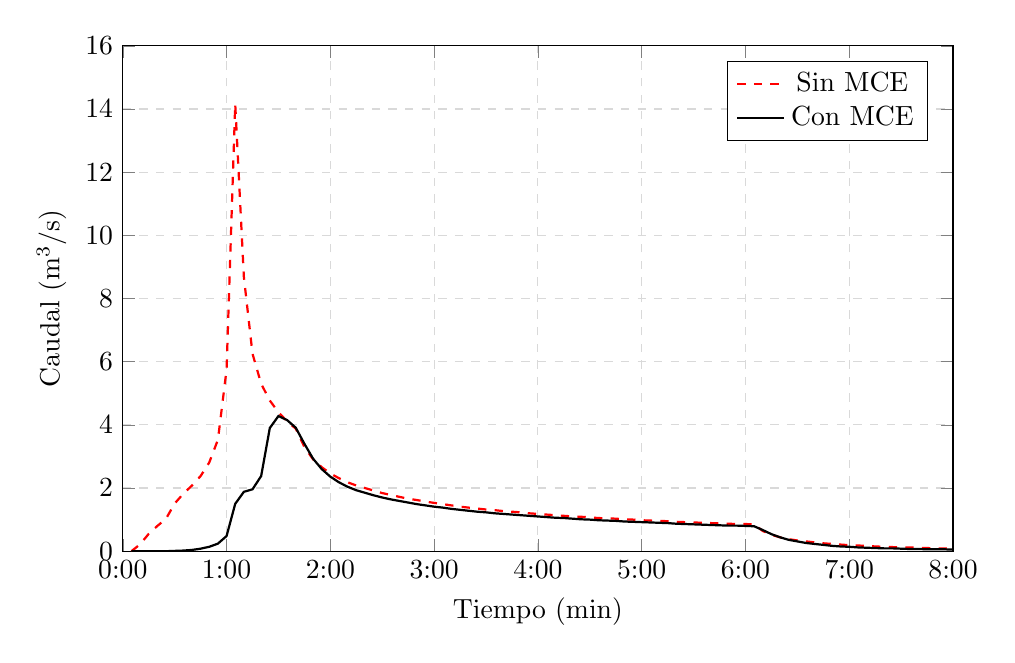
\begin{tikzpicture}
		\begin{axis}[
			width=\textwidth,
			height=8cm,
			xlabel={Tiempo (min)},
			ylabel={Caudal (m$^3$/s)},
			xmin=0,
			xmax=480,
			ymin=0,
			ymax=16,
			grid=major,
			grid style={dashed, gray!30},
			legend pos=north east,
			xtick={0, 60, 120, 180, 240, 300, 360, 420, 480},
			xticklabels={0:00, 1:00, 2:00, 3:00, 4:00, 5:00, 6:00, 7:00, 8:00},
			]
			% Sin LID
			\addplot [
			red,
			thick,
			dashed,
			] coordinates {
				(5, 0.00) (10, 0.22) (15, 0.55) (20, 0.80) (25, 1.03)
				(30, 1.51) (35, 1.82) (40, 2.08) (45, 2.38) (50, 2.81)
				(55, 3.53) (60, 5.75) (65, 14.16) (70, 8.68) (75, 6.25)
				(80, 5.30) (85, 4.77) (90, 4.40) (95, 4.11) (100, 3.88)
				(105, 3.30) (110, 2.91) (115, 2.66) (120, 2.46) (125, 2.31)
				(130, 2.18) (135, 2.08) (140, 2.00) (145, 1.92) (150, 1.84)
				(155, 1.78) (160, 1.72) (165, 1.66) (170, 1.62) (175, 1.57)
				(180, 1.53) (185, 1.49) (190, 1.45) (195, 1.41) (200, 1.38)
				(205, 1.35) (210, 1.32) (215, 1.30) (220, 1.27) (225, 1.25)
				(230, 1.23) (235, 1.20) (240, 1.18) (245, 1.16) (250, 1.14)
				(255, 1.12) (260, 1.10) (265, 1.09) (270, 1.07) (275, 1.05)
				(280, 1.04) (285, 1.03) (290, 1.01) (295, 1.00) (300, 0.98)
				(305, 0.97) (310, 0.96) (315, 0.95) (320, 0.93) (325, 0.92)
				(330, 0.91) (335, 0.90) (340, 0.89) (345, 0.88) (350, 0.87)
				(355, 0.86) (360, 0.86) (365, 0.85) (370, 0.64) (375, 0.52)
				(380, 0.44) (385, 0.38) (390, 0.34) (395, 0.31) (400, 0.28)
				(405, 0.25) (410, 0.23) (415, 0.21) (420, 0.19) (425, 0.18)
				(430, 0.17) (435, 0.15) (440, 0.14) (445, 0.13) (450, 0.12)
				(455, 0.12) (460, 0.11) (465, 0.10) (470, 0.09) (475, 0.09)
				(480, 0.08)
			};
			\addlegendentry{Sin MCE}
			
			% Con LID
			\addplot [
			black,
			thick,
			solid,
			] coordinates {
				(5, 0.00) (10, 0.00) (15, 0.00) (20, 0.00) (25, 0.00)
				(30, 0.01) (35, 0.02) (40, 0.04) (45, 0.08) (50, 0.14)
				(55, 0.24) (60, 0.48) (65, 1.50) (70, 1.88) (75, 1.96)
				(80, 2.38) (85, 3.90) (90, 4.28) (95, 4.15) (100, 3.91)
				(105, 3.40) (110, 2.93) (115, 2.60) (120, 2.36) (125, 2.18)
				(130, 2.04) (135, 1.93) (140, 1.85) (145, 1.77) (150, 1.70)
				(155, 1.64) (160, 1.59) (165, 1.54) (170, 1.49) (175, 1.45)
				(180, 1.41) (185, 1.38) (190, 1.34) (195, 1.31) (200, 1.28)
				(205, 1.25) (210, 1.23) (215, 1.20) (220, 1.18) (225, 1.16)
				(230, 1.14) (235, 1.12) (240, 1.10) (245, 1.08) (250, 1.06)
				(255, 1.05) (260, 1.03) (265, 1.01) (270, 1.00) (275, 0.98)
				(280, 0.97) (285, 0.96) (290, 0.94) (295, 0.93) (300, 0.92)
				(305, 0.91) (310, 0.90) (315, 0.89) (320, 0.87) (325, 0.86)
				(330, 0.85) (335, 0.84) (340, 0.83) (345, 0.82) (350, 0.81)
				(355, 0.81) (360, 0.80) (365, 0.79) (370, 0.67) (375, 0.54)
				(380, 0.44) (385, 0.36) (390, 0.31) (395, 0.26) (400, 0.23)
				(405, 0.20) (410, 0.17) (415, 0.15) (420, 0.14) (425, 0.12)
				(430, 0.11) (435, 0.10) (440, 0.09) (445, 0.09) (450, 0.08)
				(455, 0.07) (460, 0.07) (465, 0.06) (470, 0.06) (475, 0.06)
				(480, 0.05)
			};
			\addlegendentry{Con MCE}
			
		\end{axis}
	\end{tikzpicture}
	\caption{Comparación de hidrogramas de la subcuenca S1 con y sin medidas de control.}
	\label{fig:hidrograma_s1_comparacion}
\end{figure}

\begin{figure}[H]
	\centering
	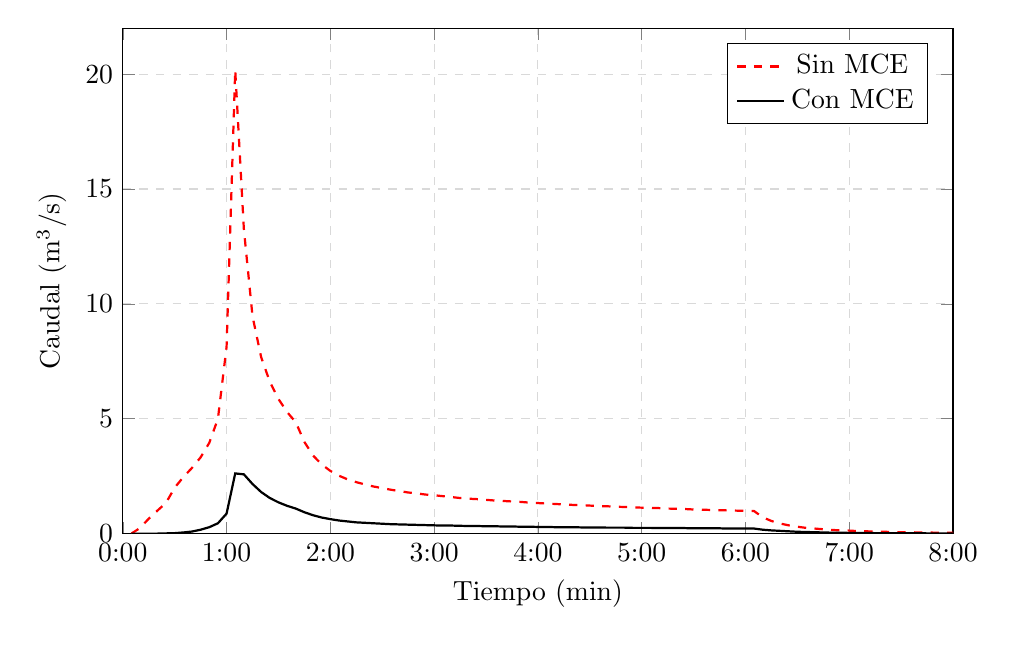
\begin{tikzpicture}
		\begin{axis}[
			width=\textwidth,
			height=8cm,
			xlabel={Tiempo (min)},
			ylabel={Caudal (m$^3$/s)},
			xmin=0,
			xmax=480,
			ymin=0,
			ymax=22,
			grid=major,
			grid style={dashed, gray!30},
			legend pos=north east,
			xtick={0, 60, 120, 180, 240, 300, 360, 420, 480},
			xticklabels={0:00, 1:00, 2:00, 3:00, 4:00, 5:00, 6:00, 7:00, 8:00},
			]
			% Sin LID
			\addplot [
			red,
			thick,
			dashed,
			] coordinates {
				(5, 0.00) (10, 0.25) (15, 0.65) (20, 1.00) (25, 1.34)
				(30, 2.00) (35, 2.46) (40, 2.86) (45, 3.32) (50, 3.95)
				(55, 5.00) (60, 8.13) (65, 20.18) (70, 13.25) (75, 9.46)
				(80, 7.68) (85, 6.61) (90, 5.86) (95, 5.29) (100, 4.85)
				(105, 3.99) (110, 3.40) (115, 3.01) (120, 2.73) (125, 2.52)
				(130, 2.36) (135, 2.24) (140, 2.14) (145, 2.05) (150, 1.98)
				(155, 1.91) (160, 1.85) (165, 1.79) (170, 1.75) (175, 1.70)
				(180, 1.67) (185, 1.63) (190, 1.59) (195, 1.55) (200, 1.52)
				(205, 1.50) (210, 1.47) (215, 1.44) (220, 1.42) (225, 1.40)
				(230, 1.38) (235, 1.35) (240, 1.33) (245, 1.31) (250, 1.29)
				(255, 1.27) (260, 1.25) (265, 1.24) (270, 1.22) (275, 1.20)
				(280, 1.19) (285, 1.17) (290, 1.16) (295, 1.14) (300, 1.13)
				(305, 1.12) (310, 1.11) (315, 1.09) (320, 1.08) (325, 1.07)
				(330, 1.05) (335, 1.04) (340, 1.03) (345, 1.02) (350, 1.01)
				(355, 1.00) (360, 0.99) (365, 0.98) (370, 0.71) (375, 0.55)
				(380, 0.44) (385, 0.36) (390, 0.30) (395, 0.25) (400, 0.22)
				(405, 0.19) (410, 0.16) (415, 0.14) (420, 0.13) (425, 0.11)
				(430, 0.10) (435, 0.09) (440, 0.08) (445, 0.07) (450, 0.06)
				(455, 0.06) (460, 0.05) (465, 0.05) (470, 0.04) (475, 0.04)
				(480, 0.04)
			};
			\addlegendentry{Sin MCE}
			
			% Con LID
			\addplot [
			black,
			thick,
			solid,
			] coordinates {
				(5, 0.00) (10, 0.00) (15, 0.00) (20, 0.00) (25, 0.01)
				(30, 0.02) (35, 0.05) (40, 0.09) (45, 0.17) (50, 0.28)
				(55, 0.45) (60, 0.87) (65, 2.62) (70, 2.58) (75, 2.16)
				(80, 1.81) (85, 1.55) (90, 1.36) (95, 1.21) (100, 1.09)
				(105, 0.93) (110, 0.80) (115, 0.70) (120, 0.63) (125, 0.57)
				(130, 0.53) (135, 0.49) (140, 0.47) (145, 0.45) (150, 0.43)
				(155, 0.41) (160, 0.40) (165, 0.39) (170, 0.38) (175, 0.37)
				(180, 0.36) (185, 0.35) (190, 0.35) (195, 0.34) (200, 0.33)
				(205, 0.33) (210, 0.32) (215, 0.32) (220, 0.31) (225, 0.31)
				(230, 0.30) (235, 0.30) (240, 0.29) (245, 0.29) (250, 0.28)
				(255, 0.28) (260, 0.28) (265, 0.27) (270, 0.27) (275, 0.27)
				(280, 0.26) (285, 0.26) (290, 0.26) (295, 0.25) (300, 0.25)
				(305, 0.25) (310, 0.24) (315, 0.24) (320, 0.24) (325, 0.24)
				(330, 0.23) (335, 0.23) (340, 0.23) (345, 0.23) (350, 0.22)
				(355, 0.22) (360, 0.22) (365, 0.22) (370, 0.17) (375, 0.14)
				(380, 0.12) (385, 0.10) (390, 0.08) (395, 0.07) (400, 0.06)
				(405, 0.05) (410, 0.04) (415, 0.04) (420, 0.03) (425, 0.03)
				(430, 0.03) (435, 0.02) (440, 0.02) (445, 0.02) (450, 0.02)
				(455, 0.02) (460, 0.02) (465, 0.01) (470, 0.01) (475, 0.01)
				(480, 0.01)
			};
			\addlegendentry{Con MCE}
			
		\end{axis}
	\end{tikzpicture}
	\caption{Comparación de hidrogramas de la subcuenca S3 con y sin medidas de control.}
	\label{fig:hidrograma_s3_comparacion}
\end{figure}


\begin{figure}[H]
	\centering
	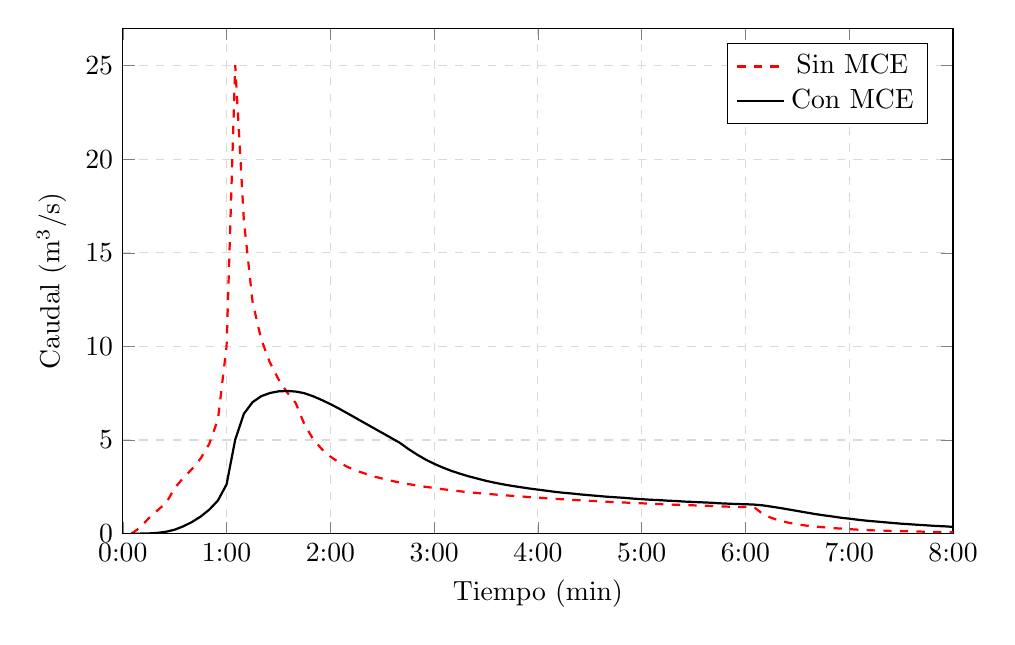
\begin{tikzpicture}
		\begin{axis}[
			width=\textwidth,
			height=8cm,
			xlabel={Tiempo (min)},
			ylabel={Caudal (m$^3$/s)},
			xmin=0,
			xmax=480,
			ymin=0,
			ymax=27,
			grid=major,
			grid style={dashed, gray!30},
			legend pos=north east,
			xtick={0, 60, 120, 180, 240, 300, 360, 420, 480},
			xticklabels={0:00, 1:00, 2:00, 3:00, 4:00, 5:00, 6:00, 7:00, 8:00},
			]
			% Sin MCE
			\addplot [
			red,
			thick,
			dashed,
			] coordinates {
				(5, 0.00) (10, 0.32) (15, 0.82) (20, 1.24) (25, 1.63)
				(30, 2.43) (35, 2.98) (40, 3.45) (45, 4.01) (50, 4.80)
				(55, 6.10) (60, 10.01) (65, 25.02) (70, 16.73) (75, 12.39)
				(80, 10.39) (85, 9.15) (90, 8.25) (95, 7.54) (100, 6.97)
				(105, 5.84) (110, 5.05) (115, 4.52) (120, 4.12) (125, 3.80)
				(130, 3.56) (135, 3.36) (140, 3.21) (145, 3.06) (150, 2.94)
				(155, 2.83) (160, 2.73) (165, 2.65) (170, 2.57) (175, 2.50)
				(180, 2.44) (185, 2.37) (190, 2.32) (195, 2.26) (200, 2.21)
				(205, 2.17) (210, 2.13) (215, 2.09) (220, 2.05) (225, 2.02)
				(230, 1.99) (235, 1.95) (240, 1.92) (245, 1.89) (250, 1.86)
				(255, 1.83) (260, 1.80) (265, 1.78) (270, 1.75) (275, 1.73)
				(280, 1.70) (285, 1.68) (290, 1.66) (295, 1.64) (300, 1.62)
				(305, 1.60) (310, 1.58) (315, 1.56) (320, 1.54) (325, 1.53)
				(330, 1.51) (335, 1.49) (340, 1.48) (345, 1.46) (350, 1.44)
				(355, 1.43) (360, 1.42) (365, 1.41) (370, 1.05) (375, 0.84)
				(380, 0.69) (385, 0.58) (390, 0.50) (395, 0.43) (400, 0.38)
				(405, 0.34) (410, 0.30) (415, 0.27) (420, 0.24) (425, 0.21)
				(430, 0.19) (435, 0.17) (440, 0.16) (445, 0.14) (450, 0.13)
				(455, 0.12) (460, 0.11) (465, 0.10) (470, 0.09) (475, 0.08)
				(480, 0.07)
			};
			\addlegendentry{Sin MCE}
			
			% Con MCE
			\addplot [
			black,
			thick,
			solid,
			] coordinates {
				(5, 0.00) (10, 0.00) (15, 0.01) (20, 0.04) (25, 0.10)
				(30, 0.21) (35, 0.39) (40, 0.62) (45, 0.91) (50, 1.28)
				(55, 1.77) (60, 2.63) (65, 5.02) (70, 6.40) (75, 7.02)
				(80, 7.34) (85, 7.51) (90, 7.60) (95, 7.62) (100, 7.59)
				(105, 7.50) (110, 7.34) (115, 7.14) (120, 6.92) (125, 6.68)
				(130, 6.42) (135, 6.16) (140, 5.90) (145, 5.64) (150, 5.38)
				(155, 5.12) (160, 4.86) (165, 4.53) (170, 4.23) (175, 3.96)
				(180, 3.73) (185, 3.53) (190, 3.35) (195, 3.20) (200, 3.06)
				(205, 2.94) (210, 2.82) (215, 2.72) (220, 2.63) (225, 2.55)
				(230, 2.48) (235, 2.41) (240, 2.35) (245, 2.29) (250, 2.23)
				(255, 2.18) (260, 2.14) (265, 2.09) (270, 2.05) (275, 2.01)
				(280, 1.97) (285, 1.94) (290, 1.91) (295, 1.87) (300, 1.84)
				(305, 1.81) (310, 1.79) (315, 1.76) (320, 1.74) (325, 1.71)
				(330, 1.69) (335, 1.67) (340, 1.65) (345, 1.62) (350, 1.60)
				(355, 1.58) (360, 1.57) (365, 1.55) (370, 1.51) (375, 1.44)
				(380, 1.37) (385, 1.29) (390, 1.21) (395, 1.13) (400, 1.05)
				(405, 0.98) (410, 0.92) (415, 0.85) (420, 0.80) (425, 0.74)
				(430, 0.69) (435, 0.65) (440, 0.61) (445, 0.57) (450, 0.53)
				(455, 0.50) (460, 0.47) (465, 0.44) (470, 0.41) (475, 0.39)
				(480, 0.36)
			};
			\addlegendentry{Con MCE}
			
		\end{axis}
	\end{tikzpicture}
	\caption{Comparación de hidrogramas de la subcuenca S5 con y sin medidas de control.}
	\label{fig:hidrograma_s5_comparacion}
\end{figure}


\begin{figure}[H]
	\centering
	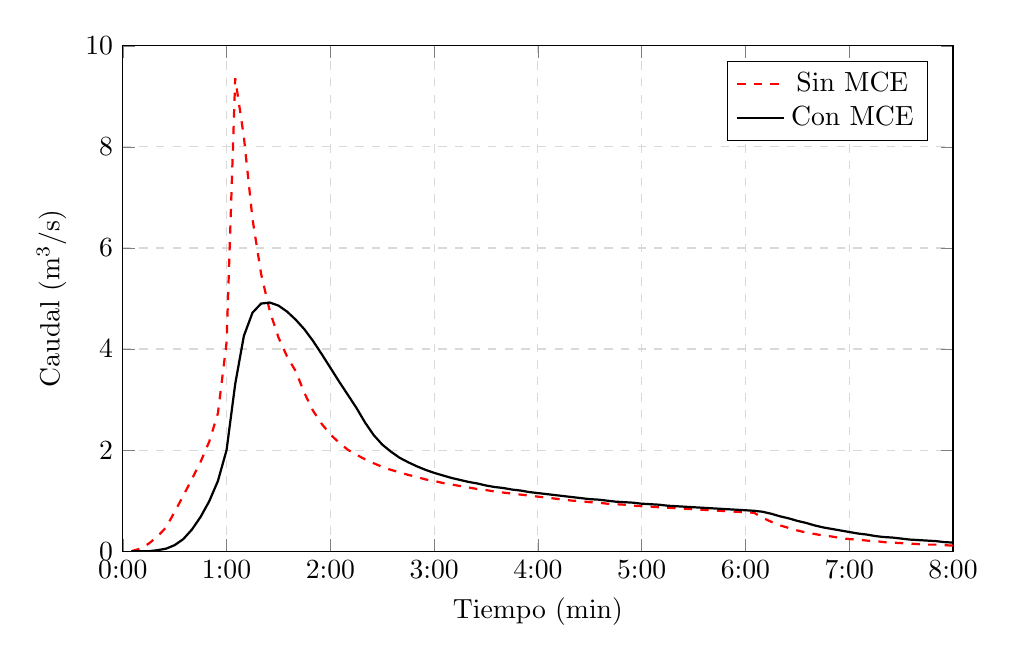
\begin{tikzpicture}
		\begin{axis}[
			width=\textwidth,
			height=8cm,
			xlabel={Tiempo (min)},
			ylabel={Caudal (m$^3$/s)},
			xmin=0,
			xmax=480,
			ymin=0,
			ymax=10,
			grid=major,
			grid style={dashed, gray!30},
			legend pos=north east,
			xtick={0, 60, 120, 180, 240, 300, 360, 420, 480},
			xticklabels={0:00, 1:00, 2:00, 3:00, 4:00, 5:00, 6:00, 7:00, 8:00},
			]
			% Sin MCE
			\addplot [
			red,
			thick,
			dashed,
			] coordinates {
				(5, 0.00) (10, 0.05) (15, 0.15) (20, 0.29) (25, 0.47)
				(30, 0.78) (35, 1.10) (40, 1.43) (45, 1.77) (50, 2.17)
				(55, 2.73) (60, 4.13) (65, 9.36) (70, 8.20) (75, 6.57)
				(80, 5.48) (85, 4.75) (90, 4.23) (95, 3.85) (100, 3.56)
				(105, 3.13) (110, 2.78) (115, 2.52) (120, 2.31) (125, 2.15)
				(130, 2.01) (135, 1.91) (140, 1.82) (145, 1.74) (150, 1.67)
				(155, 1.61) (160, 1.56) (165, 1.51) (170, 1.47) (175, 1.42)
				(180, 1.39) (185, 1.35) (190, 1.32) (195, 1.29) (200, 1.26)
				(205, 1.23) (210, 1.21) (215, 1.18) (220, 1.16) (225, 1.14)
				(230, 1.12) (235, 1.10) (240, 1.08) (245, 1.06) (250, 1.04)
				(255, 1.02) (260, 1.00) (265, 0.99) (270, 0.97) (275, 0.96)
				(280, 0.94) (285, 0.93) (290, 0.92) (295, 0.90) (300, 0.89)
				(305, 0.88) (310, 0.87) (315, 0.86) (320, 0.85) (325, 0.84)
				(330, 0.83) (335, 0.82) (340, 0.81) (345, 0.80) (350, 0.79)
				(355, 0.78) (360, 0.77) (365, 0.76) (370, 0.66) (375, 0.58)
				(380, 0.51) (385, 0.46) (390, 0.41) (395, 0.37) (400, 0.34)
				(405, 0.31) (410, 0.29) (415, 0.26) (420, 0.24) (425, 0.23)
				(430, 0.21) (435, 0.20) (440, 0.18) (445, 0.17) (450, 0.16)
				(455, 0.15) (460, 0.14) (465, 0.13) (470, 0.13) (475, 0.12)
				(480, 0.11)
			};
			\addlegendentry{Sin MCE}
			
			% Con MCE
			\addplot [
			black,
			thick,
			solid,
			] coordinates {
				(5, 0.00) (10, 0.00) (15, 0.00) (20, 0.02) (25, 0.05)
				(30, 0.12) (35, 0.24) (40, 0.43) (45, 0.68) (50, 0.99)
				(55, 1.39) (60, 2.00) (65, 3.31) (70, 4.26) (75, 4.72)
				(80, 4.90) (85, 4.92) (90, 4.86) (95, 4.74) (100, 4.58)
				(105, 4.39) (110, 4.16) (115, 3.90) (120, 3.63) (125, 3.36)
				(130, 3.10) (135, 2.84) (140, 2.55) (145, 2.30) (150, 2.11)
				(155, 1.97) (160, 1.85) (165, 1.76) (170, 1.68) (175, 1.61)
				(180, 1.55) (185, 1.50) (190, 1.45) (195, 1.41) (200, 1.37)
				(205, 1.34) (210, 1.30) (215, 1.27) (220, 1.25) (225, 1.22)
				(230, 1.20) (235, 1.17) (240, 1.15) (245, 1.13) (250, 1.11)
				(255, 1.09) (260, 1.07) (265, 1.05) (270, 1.03) (275, 1.02)
				(280, 1.00) (285, 0.98) (290, 0.97) (295, 0.96) (300, 0.94)
				(305, 0.93) (310, 0.92) (315, 0.90) (320, 0.89) (325, 0.88)
				(330, 0.87) (335, 0.86) (340, 0.85) (345, 0.84) (350, 0.83)
				(355, 0.82) (360, 0.81) (365, 0.80) (370, 0.78) (375, 0.74)
				(380, 0.69) (385, 0.65) (390, 0.60) (395, 0.56) (400, 0.51)
				(405, 0.47) (410, 0.44) (415, 0.41) (420, 0.38) (425, 0.35)
				(430, 0.33) (435, 0.30) (440, 0.28) (445, 0.27) (450, 0.25)
				(455, 0.23) (460, 0.22) (465, 0.21) (470, 0.20) (475, 0.18)
				(480, 0.17)
			};
			\addlegendentry{Con MCE}
			
		\end{axis}
	\end{tikzpicture}
	\caption{Comparación de hidrogramas de la subcuenca S6 con y sin medidas de control.}
	\label{fig:hidrograma_s6_comparacion}
\end{figure}




\begin{figure}[H]
	\centering
	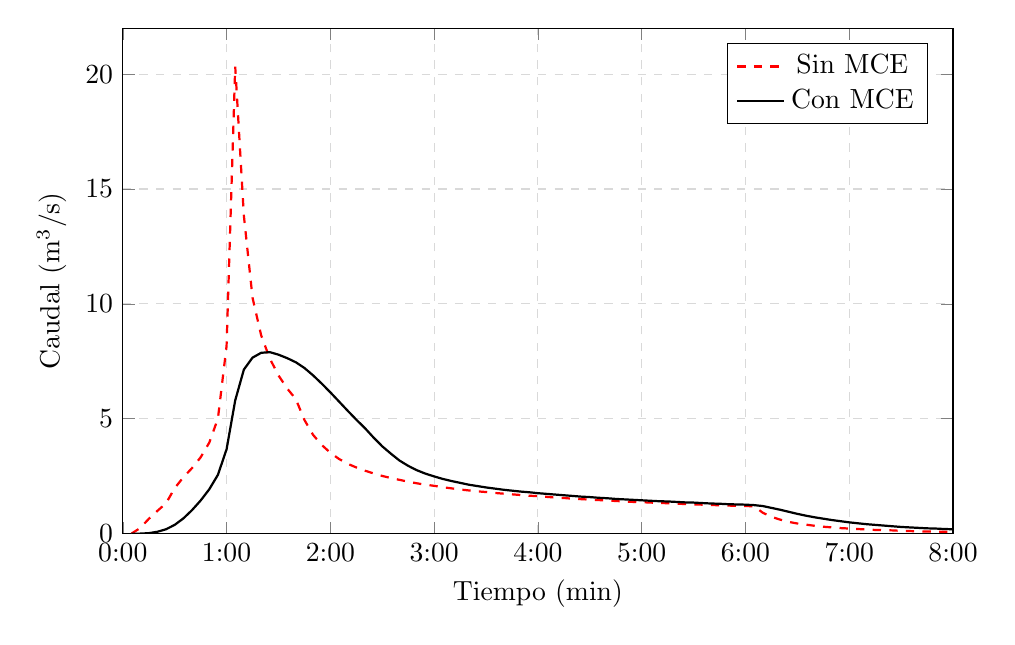
\begin{tikzpicture}
		\begin{axis}[
			width=\textwidth,
			height=8cm,
			xlabel={Tiempo (min)},
			ylabel={Caudal (m$^3$/s)},
			xmin=0,
			xmax=480,
			ymin=0,
			ymax=22,
			grid=major,
			grid style={dashed, gray!30},
			legend pos=north east,
			xtick={0, 60, 120, 180, 240, 300, 360, 420, 480},
			xticklabels={0:00, 1:00, 2:00, 3:00, 4:00, 5:00, 6:00, 7:00, 8:00},
			]
			% Sin MCE
			\addplot [
			red,
			thick,
			dashed,
			] coordinates {
				(5, 0.00) (10, 0.24) (15, 0.64) (20, 0.99) (25, 1.32)
				(30, 1.98) (35, 2.45) (40, 2.85) (45, 3.32) (50, 3.96)
				(55, 5.01) (60, 8.17) (65, 20.33) (70, 13.84) (75, 10.27)
				(80, 8.63) (85, 7.62) (90, 6.89) (95, 6.32) (100, 5.86)
				(105, 4.95) (110, 4.30) (115, 3.86) (120, 3.52) (125, 3.25)
				(130, 3.04) (135, 2.88) (140, 2.74) (145, 2.62) (150, 2.51)
				(155, 2.42) (160, 2.34) (165, 2.26) (170, 2.19) (175, 2.13)
				(180, 2.08) (185, 2.02) (190, 1.97) (195, 1.92) (200, 1.88)
				(205, 1.84) (210, 1.81) (215, 1.77) (220, 1.74) (225, 1.71)
				(230, 1.68) (235, 1.65) (240, 1.63) (245, 1.60) (250, 1.57)
				(255, 1.55) (260, 1.52) (265, 1.50) (270, 1.48) (275, 1.46)
				(280, 1.44) (285, 1.42) (290, 1.40) (295, 1.38) (300, 1.37)
				(305, 1.35) (310, 1.34) (315, 1.32) (320, 1.30) (325, 1.29)
				(330, 1.27) (335, 1.26) (340, 1.25) (345, 1.23) (350, 1.22)
				(355, 1.21) (360, 1.20) (365, 1.19) (370, 0.91) (375, 0.73)
				(380, 0.61) (385, 0.51) (390, 0.44) (395, 0.39) (400, 0.34)
				(405, 0.30) (410, 0.27) (415, 0.24) (420, 0.22) (425, 0.20)
				(430, 0.18) (435, 0.16) (440, 0.15) (445, 0.14) (450, 0.12)
				(455, 0.11) (460, 0.10) (465, 0.09) (470, 0.09) (475, 0.08)
				(480, 0.07)
			};
			\addlegendentry{Sin MCE}
			
			% Con MCE
			\addplot [
			black,
			thick,
			solid,
			] coordinates {
				(5, 0.00) (10, 0.00) (15, 0.02) (20, 0.08) (25, 0.19)
				(30, 0.38) (35, 0.66) (40, 1.02) (45, 1.44) (50, 1.93)
				(55, 2.56) (60, 3.67) (65, 5.80) (70, 7.14) (75, 7.66)
				(80, 7.87) (85, 7.90) (90, 7.79) (95, 7.64) (100, 7.46)
				(105, 7.21) (110, 6.89) (115, 6.53) (120, 6.15) (125, 5.75)
				(130, 5.35) (135, 4.96) (140, 4.59) (145, 4.18) (150, 3.80)
				(155, 3.48) (160, 3.18) (165, 2.95) (170, 2.76) (175, 2.61)
				(180, 2.49) (185, 2.38) (190, 2.29) (195, 2.21) (200, 2.13)
				(205, 2.07) (210, 2.01) (215, 1.96) (220, 1.91) (225, 1.87)
				(230, 1.83) (235, 1.80) (240, 1.76) (245, 1.73) (250, 1.70)
				(255, 1.67) (260, 1.64) (265, 1.61) (270, 1.59) (275, 1.56)
				(280, 1.54) (285, 1.51) (290, 1.49) (295, 1.47) (300, 1.45)
				(305, 1.43) (310, 1.41) (315, 1.40) (320, 1.38) (325, 1.36)
				(330, 1.35) (335, 1.33) (340, 1.31) (345, 1.30) (350, 1.28)
				(355, 1.27) (360, 1.26) (365, 1.24) (370, 1.20) (375, 1.12)
				(380, 1.04) (385, 0.95) (390, 0.86) (395, 0.78) (400, 0.71)
				(405, 0.65) (410, 0.59) (415, 0.54) (420, 0.49) (425, 0.45)
				(430, 0.41) (435, 0.38) (440, 0.35) (445, 0.32) (450, 0.29)
				(455, 0.27) (460, 0.25) (465, 0.23) (470, 0.22) (475, 0.20)
				(480, 0.19)
			};
			\addlegendentry{Con MCE}
			
		\end{axis}
	\end{tikzpicture}
	\caption{Comparación de hidrogramas de la subcuenca S7 con y sin medidas de control.}
	\label{fig:hidrograma_s7_comparacion}
\end{figure}


\begin{figure}[H]
	\centering
	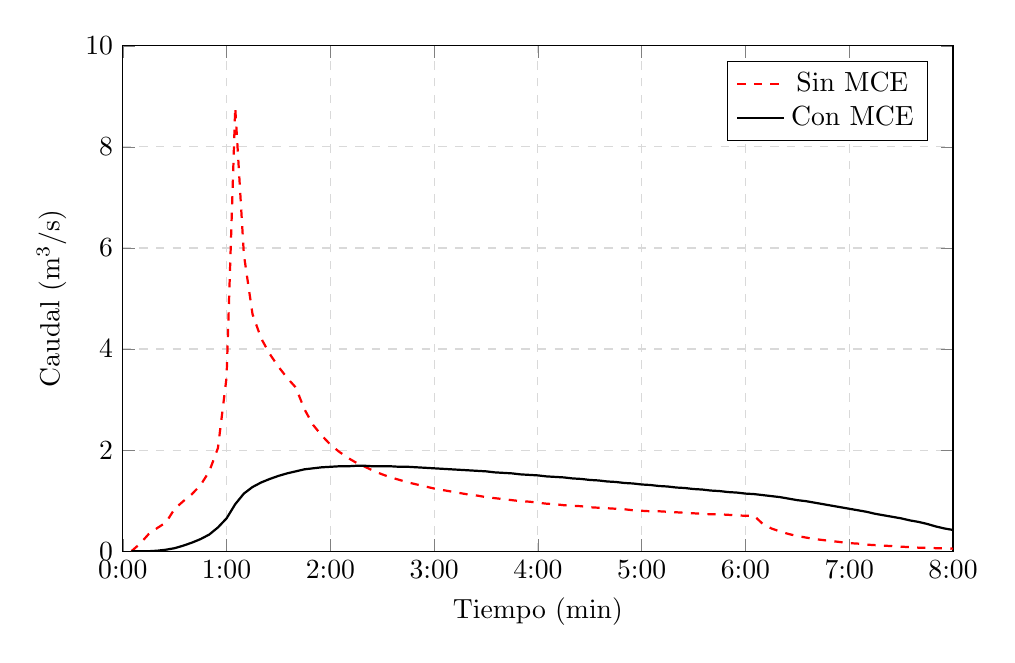
\begin{tikzpicture}
		\begin{axis}[
			width=\textwidth,
			height=8cm,
			xlabel={Tiempo (min)},
			ylabel={Caudal (m$^3$/s)},
			xmin=0,
			xmax=480,
			ymin=0,
			ymax=10,
			grid=major,
			grid style={dashed, gray!30},
			legend pos=north east,
			xtick={0, 60, 120, 180, 240, 300, 360, 420, 480},
			xticklabels={0:00, 1:00, 2:00, 3:00, 4:00, 5:00, 6:00, 7:00, 8:00},
			]
			% Sin MCE
			\addplot [
			red,
			thick,
			dashed,
			] coordinates {
				(5, 0.00) (10, 0.15) (15, 0.34) (20, 0.46) (25, 0.57)
				(30, 0.84) (35, 0.99) (40, 1.13) (45, 1.31) (50, 1.58)
				(55, 2.04) (60, 3.44) (65, 8.78) (70, 5.87) (75, 4.69)
				(80, 4.21) (85, 3.90) (90, 3.65) (95, 3.43) (100, 3.24)
				(105, 2.81) (110, 2.50) (115, 2.29) (120, 2.11) (125, 1.97)
				(130, 1.85) (135, 1.75) (140, 1.67) (145, 1.59) (150, 1.52)
				(155, 1.46) (160, 1.41) (165, 1.36) (170, 1.32) (175, 1.28)
				(180, 1.24) (185, 1.21) (190, 1.18) (195, 1.15) (200, 1.12)
				(205, 1.10) (210, 1.07) (215, 1.05) (220, 1.03) (225, 1.01)
				(230, 0.99) (235, 0.98) (240, 0.96) (245, 0.94) (250, 0.93)
				(255, 0.91) (260, 0.90) (265, 0.89) (270, 0.87) (275, 0.86)
				(280, 0.85) (285, 0.84) (290, 0.83) (295, 0.81) (300, 0.80)
				(305, 0.79) (310, 0.79) (315, 0.78) (320, 0.77) (325, 0.76)
				(330, 0.75) (335, 0.74) (340, 0.73) (345, 0.73) (350, 0.72)
				(355, 0.71) (360, 0.70) (365, 0.70) (370, 0.54) (375, 0.45)
				(380, 0.39) (385, 0.34) (390, 0.30) (395, 0.27) (400, 0.24)
				(405, 0.22) (410, 0.20) (415, 0.18) (420, 0.16) (425, 0.15)
				(430, 0.13) (435, 0.12) (440, 0.11) (445, 0.10) (450, 0.09)
				(455, 0.08) (460, 0.07) (465, 0.07) (470, 0.06) (475, 0.06)
				(480, 0.05)
			};
			\addlegendentry{Sin MCE}
			
			% Con MCE
			\addplot [
			black,
			thick,
			solid,
			] coordinates {
				(5, 0.00) (10, 0.00) (15, 0.00) (20, 0.01) (25, 0.03)
				(30, 0.06) (35, 0.11) (40, 0.17) (45, 0.24) (50, 0.33)
				(55, 0.47) (60, 0.65) (65, 0.93) (70, 1.14) (75, 1.27)
				(80, 1.36) (85, 1.43) (90, 1.49) (95, 1.54) (100, 1.58)
				(105, 1.62) (110, 1.64) (115, 1.66) (120, 1.67) (125, 1.68)
				(130, 1.68) (135, 1.69) (140, 1.69) (145, 1.68) (150, 1.68)
				(155, 1.68) (160, 1.67) (165, 1.67) (170, 1.66) (175, 1.65)
				(180, 1.64) (185, 1.63) (190, 1.62) (195, 1.61) (200, 1.60)
				(205, 1.59) (210, 1.58) (215, 1.56) (220, 1.55) (225, 1.54)
				(230, 1.52) (235, 1.51) (240, 1.50) (245, 1.48) (250, 1.47)
				(255, 1.46) (260, 1.44) (265, 1.43) (270, 1.41) (275, 1.40)
				(280, 1.38) (285, 1.37) (290, 1.35) (295, 1.34) (300, 1.32)
				(305, 1.31) (310, 1.29) (315, 1.28) (320, 1.26) (325, 1.25)
				(330, 1.23) (335, 1.22) (340, 1.20) (345, 1.19) (350, 1.17)
				(355, 1.16) (360, 1.14) (365, 1.13) (370, 1.11) (375, 1.09)
				(380, 1.07) (385, 1.04) (390, 1.01) (395, 0.99) (400, 0.96)
				(405, 0.93) (410, 0.90) (415, 0.87) (420, 0.84) (425, 0.81)
				(430, 0.78) (435, 0.74) (440, 0.71) (445, 0.68) (450, 0.65)
				(455, 0.61) (460, 0.58) (465, 0.54) (470, 0.49) (475, 0.45)
				(480, 0.42)
			};
			\addlegendentry{Con MCE}
			
		\end{axis}
	\end{tikzpicture}
	\caption{Comparación de hidrogramas de la subcuenca S8 con y sin medidas de control.}
	\label{fig:hidrograma_s8_comparacion}
\end{figure}